\blankpage

\thispagestyle{empty}
\clearpage
\begin{tikzpicture}[remember picture, overlay]
\node at (3,-7) {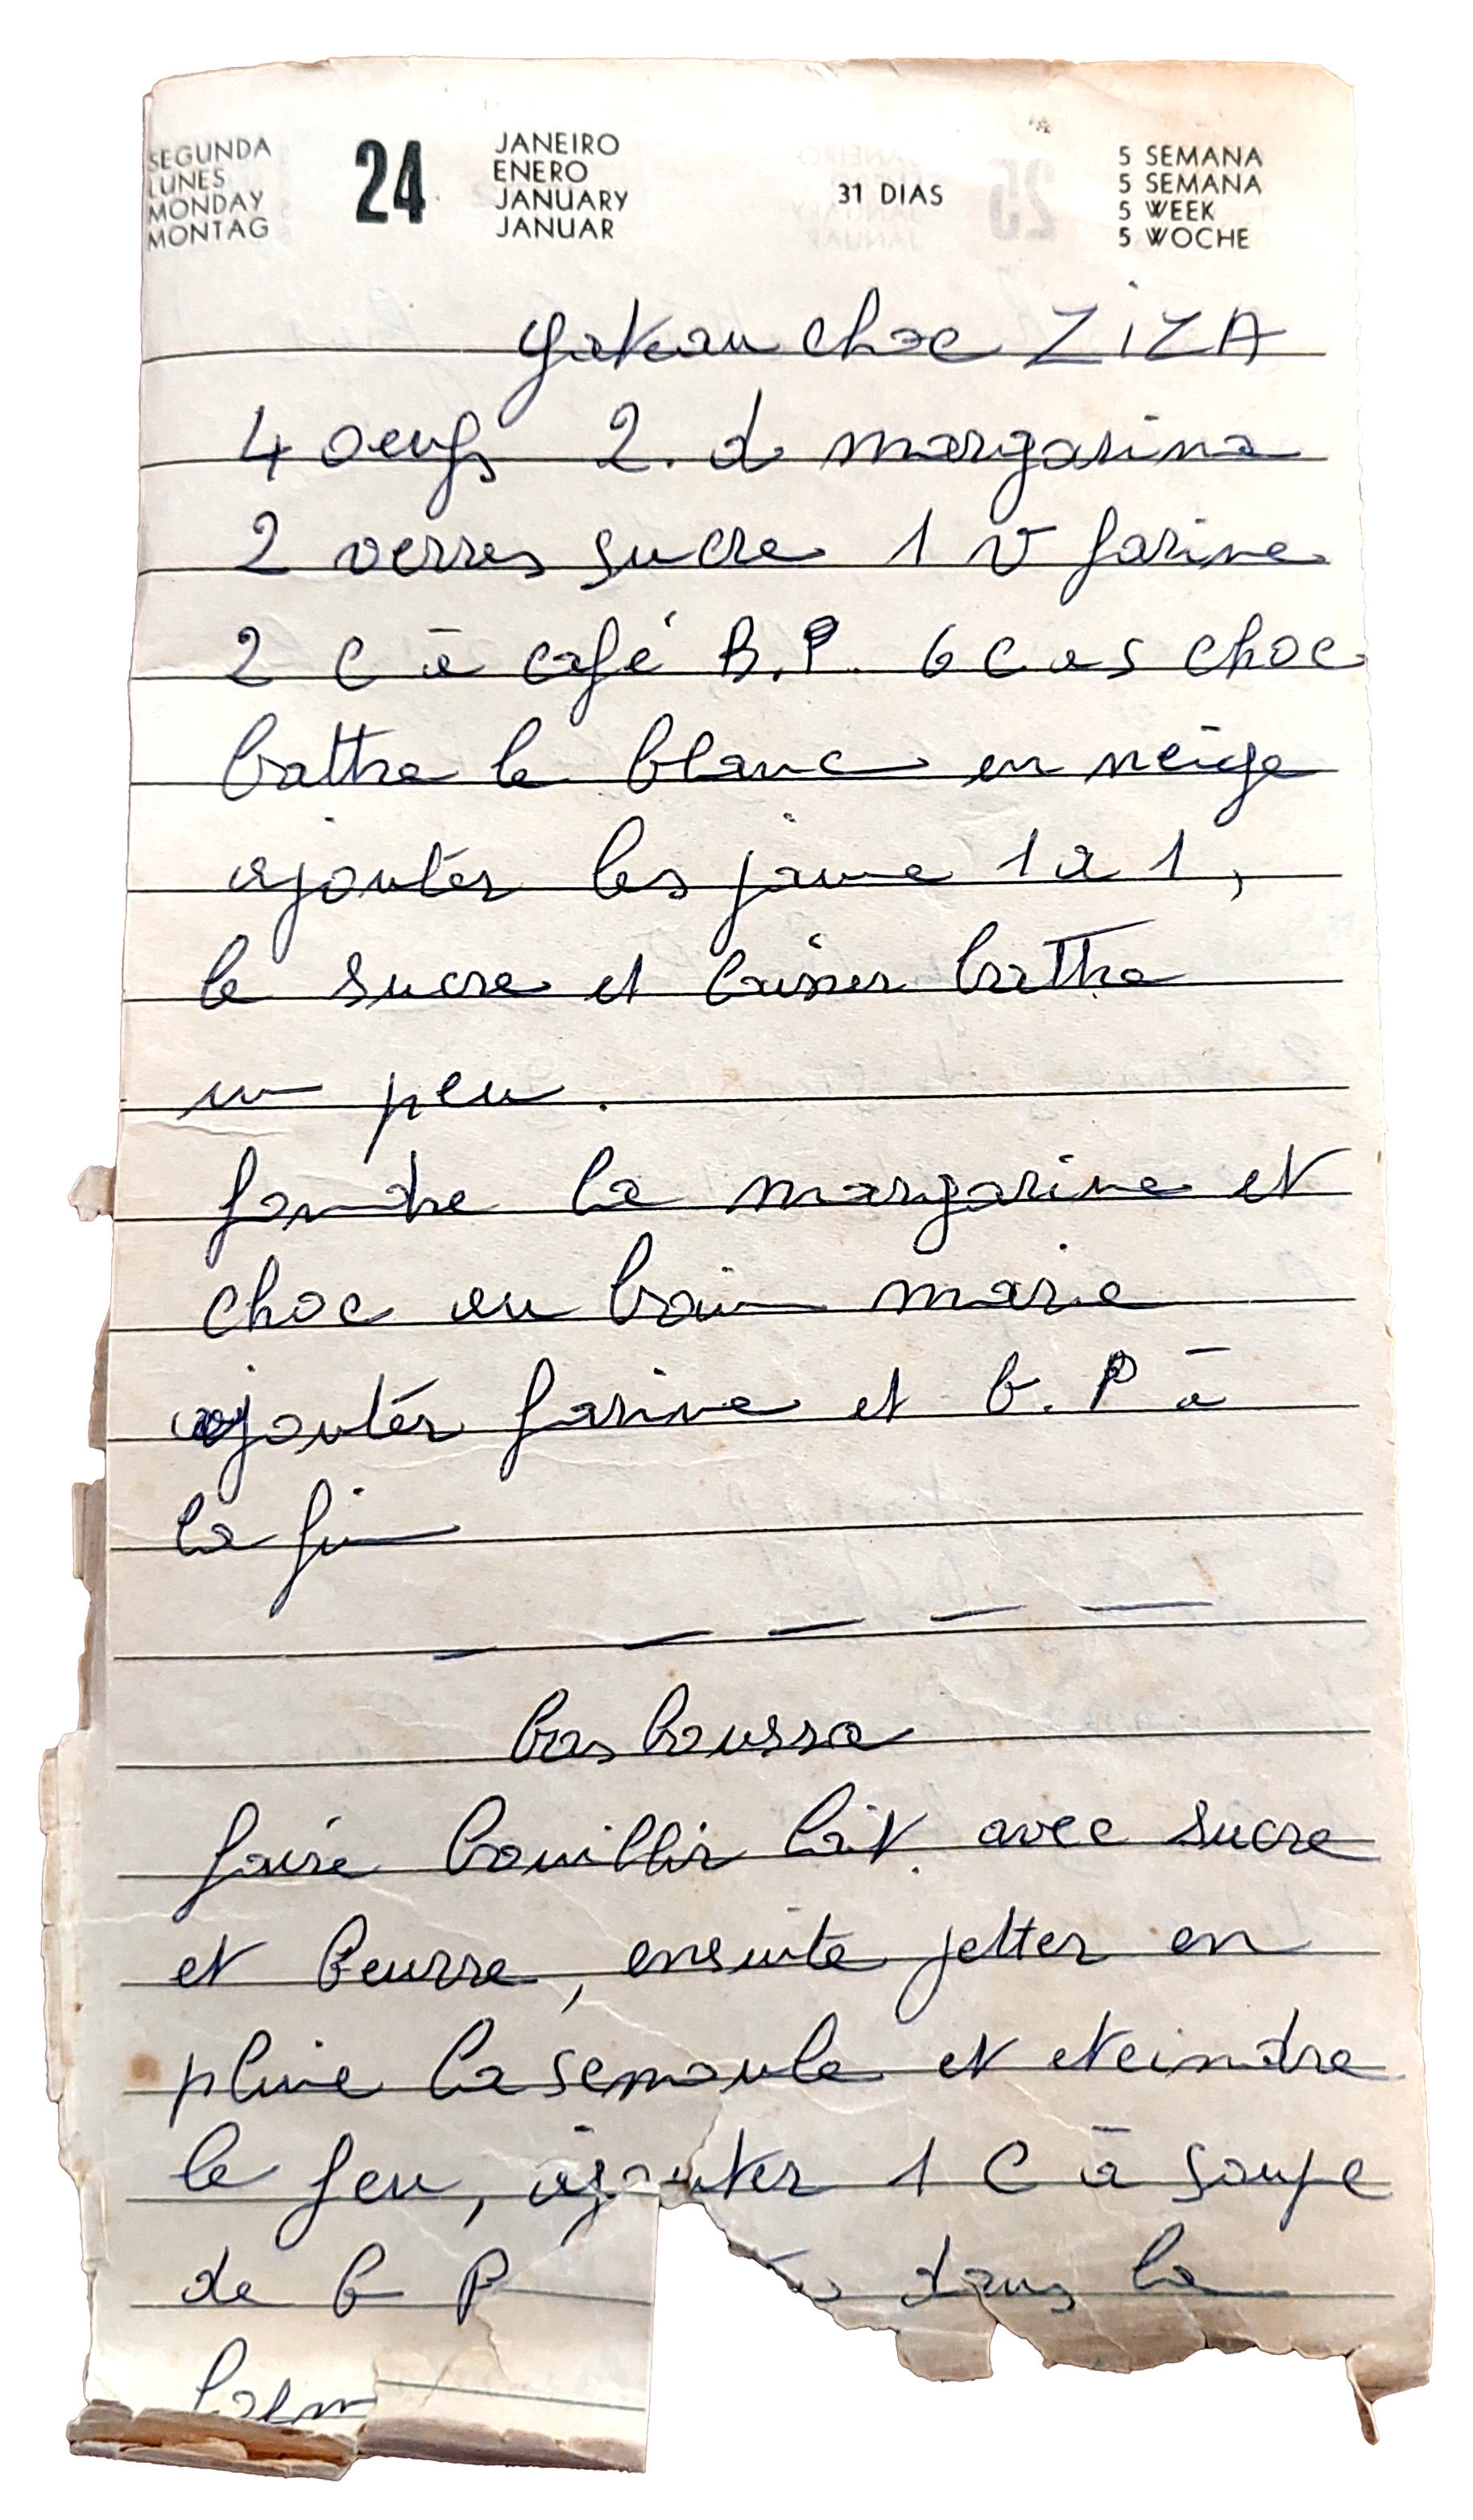
\includegraphics[width=8cm]{./recettes/edités/Gateau choc Ziza, Basboussa et Atayef (parte 1).jpg}}; 
\end{tikzpicture}\clearpage\thispagestyle{empty}
% \begin{tikzpicture}[remember picture,overlay]
% \fill[black] (-3,3.5) rectangle (14,-21.5);
% \end{tikzpicture}
\clearpage

\chapter*{Basboussa}

\section{Ingrédients originaux}

\begin{itemize}
\item Lait, sucre et beurre
\item Semoule
\item 1 c à soupe de \textsc{b.p.}
\item Pour le sirop:
	\begin{itemize}
	\item 3 verres de sucre
	\item 2 verres d’eau
	\item 1/2 citron
	\item 1 c à soupe vinaigre
	\end{itemize}
\end{itemize}

\section{Préparation adaptée}

Faites bouillir le lait avec le sucre et le beurre, versez la semoule en pluie en remuant puis retirez du feu ; laissez tiédir, ajoutez la levure chimique et mélangez. Versez dans un moule beurré et faites cuire à 180°\,\textsc{c} pendant 30--40 minutes, jusqu’à ce que le dessus soit doré ; préparez le sirop en faisant bouillir le sucre, l’eau et le citron (le vinaigre est facultatif) et, à la sortie du four, arrosez le gâteau encore chaud en laissant absorber avant de servir.

\chapter{Bolo de semolina}

\section{Ingredientes originais}

\begin{itemize}
\item Leite, açúcar e manteiga
\item Sêmola
\item 1 colher de sopa de fermento químico
\item Para a calda:
	\begin{itemize}
	\item 3 copos de açúcar
	\item 2 copos de água
	\item 1/2 limão
	\item 1 colher de sopa de vinagre
	\end{itemize}
\end{itemize}

\section{Modo de preparo adaptado}

Ferva o leite com o açúcar e a manteiga, despeje a sêmola em chuva mexendo e retire do fogo; deixe amornar, adicione o fermento químico e misture. Coloque em forma untada e asse a 180°\,\textsc{c} por 30--40 minutos, até dourar; prepare a calda fervendo açúcar, água e limão (vinagre opcional) e, ao retirar do forno, regue o bolo ainda quente, deixando absorver antes de servir.